% !Mode:: "TeX:UTF-8"
\documentclass{article}
\usepackage{lastpage} % Required to determine the last page for the footer
\usepackage{extramarks} % Required for headers and footers
\usepackage{graphicx} % Required to insert images
\usepackage{listings} % Required for insertion of code
\usepackage[usenames,dvipsnames]{color} % Required for custom colors
\usepackage{amsmath,amsthm}
\usepackage{courier} % Required for the courier font
\usepackage{enumerate}
\usepackage{algorithm}
\usepackage{algorithmic}
\usepackage{algpseudocode}
\usepackage{supertabular}
% Margins
\linespread{1.3} % Line spacing
% Set up the header and footer

%----------------------------------------------------------------------------------
%   CODE INCLUSION CONFIGURATION
%----------------------------------------------------------------------------------------
\definecolor{MyDarkGreen}{rgb}{0.0,0.4,0.0} % This is the color used for comments
\lstloadlanguages{Python} % Load Perl syntax for listings, for a list of other languages supported see: ftp://ftp.tex.ac.uk/tex-archive/macros/latex/contrib/listings/listings.pdf
\lstset{language=Python, % Use Perl in this example
        %frame=single, % Single frame around code
        basicstyle=\small\ttfamily, % Use small true type font
        keywordstyle=[1]\color{Blue}\bf, % Perl functions bold and blue
        keywordstyle=[2]\color{Purple}, % Perl function arguments purple
        keywordstyle=[3]\color{Blue}\underbar, % Custom functions underlined and blue
        identifierstyle=, % Nothing special about identifiers
        commentstyle=\usefont{T1}{pcr}{m}{sl}\color{MyDarkGreen}\small, % Comments small dark green courier font
        stringstyle=\color{Purple}, % Strings are purple
        showstringspaces=false, % Don't put marks in string spaces
        tabsize=3, % 5 spaces per tab
        %
        % Put standard Perl functions not included in the default language here
        morekeywords={rand},
        %
        % Put Perl function parameters here
        morekeywords=[2]{on, off, interp},
        %
        % Put user defined functions here
        morekeywords=[3]{test},
        %
        morecomment=[l][\color{Blue}]{...}, % Line continuation (...) like blue comment
        numbers=left, % Line numbers on left
        firstnumber=1, % Line numbers start with line 1
        numberstyle=\tiny\color{Blue}, % Line numbers are blue and small
        stepnumber=5 % Line numbers go in steps of 5
}

% Creates a new command to include a python script, the first parameter is the filename of the script (without .py), the second parameter is the caption
\newcommand{\pythonscript}[2]{
\begin{itemize}
\item[]\lstinputlisting[caption=#2,label=#1]{#1.py}
\end{itemize}
}

%----------------------------------------------------------------------------------------
%   NAME AND CLASS SECTION
%----------------------------------------------------------------------------------------

\newcommand{\hmwkTitle}{Assignment\ \#5} % Assignment title
\newcommand{\hmwkDueDate}{Friday,\ Dec \ 18,\ 2015} % Due date
\newcommand{\hmwkClass}{CS091M4041H\ 101} % Course/class
\newcommand{\hmwkClassTime}{9:20am} % Class/lecture time
\newcommand{\hmwkClassInstructor}{Dongbo Bu} % Teacher/lecturer
\newcommand{\hmwkAuthorName}{cwlseu} % Your name

\numberwithin{equation}{section}
%----------------------------------------------------------------------------------------
%   TITLE PAGE
%----------------------------------------------------------------------------------------

\title{
\vspace{2in}
\textmd{\textbf{\hmwkClass:\ \hmwkTitle}}\\
\normalsize\vspace{0.1in}\small{Due\ on\ \hmwkDueDate}\\
\vspace{0.1in}\large{\textit{\hmwkClassInstructor\ \hmwkClassTime}}
\vspace{3in}
}

\author{\textbf{\hmwkAuthorName}\\\textbf{\hmwkAuthorStuID}}
\date{} % Insert date here if you want it to appear below your name

\begin{document}

\maketitle
\newpage


%
% Problem 1
%
\section{Problem Reduction}
Support the you are a matchmaker and there are some boys and girls. 
Since the boys are alway more than girls, you can assume that 
if a girl express her love to a boy , the boy will always accept her. 
Now you know every girl’s thought(a girl may like more than one boy) and 
you want to make as much pairs as you can. show that you can do this 
using maximum flow algorithm.
    \subsection{Algorithm}
    This is a matching problem. All the girls and boys could be doneted as $v_i$, all $v_i \in V$. 
    In addition, we will add $2$ extra nodes $s$ and $t$. $s$ have edge direct at all the girls vertices. 
    And all the boys vertices have one edge direct at the $t$ nodes. 
    We could find the max flow of the $direct-graph$. The max flow is the maximal matching.
    \begin{center}
            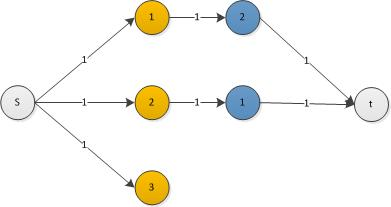
\includegraphics[width=0.75\columnwidth]{boysgirlsmatching} % Example image
    \end{center} 
    In the network graph, the yellow vertices is girls and the blue vertices denote boys.The white vertices $s$ and $t$ is extra nodes. From the yellow node direct at blue node means the girl love the boy. We could find the max flow from the network which is the max number of matching pairs.
    \subsection{Time Complexity}
    All the edges capacity $C(e) = {0|1}$,So the time complexity is $O(mn)$, $m$ is number of girls and $n$ is the number of boys.
%
% Problem 2
%
\section{Problem Reduction}
There is a matrix filled with 0 and 1, you know the sum of every row and column. you are asked to give such a matrix which satisfy the conditions.
    \subsection{Algorithm}
    The problem could be model as a $Push-Relabel$ problem. The sum of row could be denote as set $L$
and the sum of column denote as set $R$. In $L$, every element  have been set value that sum of the row. The same as $R$, every element have value that the sum of the column. Adding a source vertices $s$ direct at all element in $L$, and adding a tink vertice $t$ which at all element in $R$ dircet. Otherwise, all the element in $L$ adjacent to all element from $R$, the weight is 0 or 1. In the network, find a path from $s$ to $t$. If we could find a path from $s$ to $t$, then the input matrix have solution.

    \begin{center}
            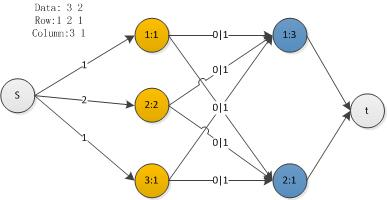
\includegraphics[width=0.75\columnwidth]{rowcolumn} % Example image
    \end{center} 
    In the network graph, the yellow vertices is row sum and the blue vertices denote column sum.The white vertices $s$ and $t$ is extra nodes. The solution is find a $s - t$ path in the network.
    \subsection{Time Complexity}
    The time complexity is $O(mn^2)$
%
% Problem 3
%

\section{Dogs and kennels}
On a grid map there are n little dogs and n kennels. In each unit time,
every little dog can move one unit step, either horizontally, or vertically, to
an adjacent point. For each little dog, you need to pay a 1 travel fee for
every step it moves, until it enters a kennel. The task is complicated with
the restriction that each kennel can accommodate only one little dog.\\
Give a polynomial-time algorithm to compute the minimum amount of
money you need to pay in order to send these n little dogs into those n
different kennels.
    \subsection{Algorithm}
    The problem is minimize cost flow problem.The dogs point is the goods supplier, and the kennels is denote as Supermarket. Now we should find the minimum cost for supplier send goods to Supermarket.In this problem, we could add extra vertices $s$ as headquarter of all the suppliers and add $t$ as headquarter of all the supermarket. We could use Klein algorithm to solve the minimum cost flow algorithm.
    \subsection{Algorithm}
    \alglanguage{pseudocode}
    \begin{algorithm}
    \caption{Klein algorithm}
    \label{alg1}
        \begin{algorithmic}[1]
            \STATE Finding  a flow $f$ with value $w_0$ using maximum-flow algorithm say Ford-Fulkerson    
            \LOOP
                \IF{$N'(f)$ contains a cycle C with negative cost  $do$}
                    \STATE Donate $b$ as the bottleneck of cycle C
                    \STATE Define $ff$ as the flow along C
                    \STATE $f \gets f + b*ff$ 
                \ENDIF
            \ENDLOOP
            \RETURN $f$
        \end{algorithmic}
    \end{algorithm}
    The cycle with negative cost can be found using Bellman-Ford algorithm.

%
% Problem 4
%
\section{Unique Cut}
Let $G = (V,E)$ be a directed graph, with source s \in V , sink t \in V , and
nonnegative edge capacities $c_e$. Give a polynomial-time algorithm to decide
whether $G$ has a unique minimum st cut.
    \subsection{Algorithm}
    The algorithm is based on Ford\_Fulkerson algorithm.

        \begin{algorithm}
            \caption{Unique-Cut-Or-Not}
            \label{alg2}
            \begin{algorithmic}[1]
                \STATE {$minCut$ \gets  $empty set$}
                \STATE {$maxFlow$ \gets $Ford\_Fulkerson find max flow and minCut update$}
                \FOR{$e \gets minCut.pop()$} 
                     \STATE increase the C(e)
                     \IF{$maxFlow \eq new Graph to Ford\_Fulkerson$}
                        \RETURN $FALSE$
                     \ENDIF
                \ENDFOR
                \RETURN $TURE$
            \end{algorithmic}
        \end{algorithm}
    \subsection{Correctness}
    If we increase bottle edges weight in the set of min cut, the max flow didn't change, we could say the edge have substitute edges, so the minimum s-t cut isn't unique. On the contrary, if we increase a min cut edge, the max flow have change, so the minimum cut is unique.
    \subsection{Time Complexity}
    The time complexity is the product of the size of minCut and the time complexity of Ford\_Fulkerson algorithm. $T(n) = s*T(Ford\_Fulkerson) < O(m^2C)$.The time complexity is $O(m^2C)$.
%
% Execise 1
%
\section{Ford-Fulkerson}
Implement Ford-Fulkerson algorithm to find the maximum flow of the following network, and list your intermediate steps. Use you implementation
to solve problem 1 and show your answers.\\
\emph{INPUT}: Number of girls and boys. the boys that each girl likes. see more
detial in the file problem1.data.\\
\emph{OUTPUT}: Number of pairs you can make.
    \subsection{Algorithm}
        \pythonscript{Ford_Fulkserson}{Ford\_Fulkserson Algorithm using python implement}

    \subsection{Result}
    \newpage
        \begin{table}[tbp]     
            \centering 
                \begin{tabular}{ccc}  
                \hline
                    Girls & Boys & match number  \\ 
                \hline  % \hline 在此行下面画一横线
                    3  & 2 & 2  \\
                    10 & 10 & 9 \\
                    11 & 17 & 11 \\
                    17 & 19 & 16 \\
                    21 & 27 & 18 \\
                    117 & 119 & 116 \\
                    \hline
                \end{tabular}
            \caption{Average running time with different method.}
        \end{table}
%
% Execise 2
%
\section{Push-Relabel}
Implement push-relabel algorithm to find the maximum flow of a network, and list your intermediate steps. Use your implementation to solve problem 2 and write a check problem to see if your answer is right.\\
\emph{INPUT}: Numbers of rows and columns. And the sum of them. See more detial in the file problem2.data. e.g.\\
10 10 \\
5 5 7 7 6 3 5 7 7 3 \\
6 6 7 4 5 6 6 4 4 7 \\
\emph{OUTPUT}: The matrix you get. Any one satisfy the conditions will be accept.

\subsection{Algorithm}
        \pythonscript{Push_Relabel}{Push\_Relabel Algorithm using python implement}
\subsection{Result}
        the max flow:  55  the matrix exist: True\\
        the max flow:  94  the matrix exist: True\\
        the max flow:  6684  the matrix exist: True\\
        the max flow:  650  the matrix exist: True\\
        the max flow:  1243  the matrix exist: True\\
        the max flow:  5603  the matrix exist: True\\
        the max flow:  502  the matrix exist: True\\
        the max flow:  118  the matrix exist: True\\
        the max flow:  221  the matrix exist: True\\
\end{document}